%!LW recipe=lualatex->biber->lualatex
\documentclass[11pt]{article}

% PACKAGES --------------------------------------------------

\usepackage{geometry}
\usepackage{fontspec}
\usepackage{indentfirst}
\usepackage{tabularx}
\usepackage{graphicx}
\usepackage{enumitem}
\usepackage{hyperref}
\usepackage[style=numeric, backend=biber]{biblatex}
\usepackage{amsmath,amssymb,amsfonts, bm}
\usepackage{booktabs}
\usepackage{setspace}
\usepackage{fancyhdr}
\usepackage{titlesec}
\usepackage{siunitx}
\usepackage{wrapfig}
\usepackage{float}

% SETTINGS --------------------------------------------------

    \geometry{letterpaper}
    \geometry{left=2.54cm, right=2.39cm, top=1.9cm, bottom=1.9cm, includeheadfoot, headheight=19.27817pt}

    \doublespace{}
    \addbibresource{lab1.bib}
    \emergencystretch=1em

    \pagestyle{fancy}
    \fancyhf{}
    \fancyhead[L]{\textbf{BME282 --- Lab: Mechanical Properties}}
    \fancyfoot[C]{\textbf{-\ \thepage\ -}}
    \renewcommand{\headrulewidth}{1.5pt}
    \renewcommand{\headruleskip}{1ex}

    \titleformat{\section}
        {\normalfont\normalsize\bfseries\uppercase}{\thesection}{1em}{}
    \titleformat{\subsection}
    {\normalfont\normalsize\bfseries}{\thesubsection}{1em}{}

% MAIN --------------------------------------------------

\begin{document}
    
    \newgeometry{left=2.54cm, right=2.39cm, top=1.9cm, bottom=1.9cm}
\begin{titlepage}
    \noindent
    \begin{minipage}{\textwidth}
        \setlength{\intextsep}{0pt}%
        \setlength{\columnsep}{0pt}%
        \begin{wrapfigure}{tr}{1in}
            \centering
            
\includegraphics[width=\linewidth]{UWaterloo_Management_Sci_Logo_vert_rgb}
        \end{wrapfigure}

        \noindent\textbf{University of Waterloo --- Department of Systems Design}
    \end{minipage}

    \vspace*{1.25in}

    \begin{center}
        \centerline{\rule{\textwidth}{1pt}}

        \textbf{
            \Large
            BME282 --- Materials Science for Biomedical Engineers\\
            Lab --- Mechanical Properties
        }

        \centerline{\rule{\textwidth}{1pt}}
        
        \vspace*{1.5in}
        Prepared for:\\
        Prof.\ Biro

        \vfill

        Group 9\\
        \bigskip
        Jamie Kang\\
        Grace Hur\\
        Myesha Zaman\\
        Jaime Thrower\\
        \vspace*{0.5in}
        Novermber 21, 2023
    \end{center}
 \end{titlepage}
\restoregeometry{}
    \tableofcontents
    \newpage

    \section{Summary}
        \subsection{Purpose}
            Understanding the properties of a material is essential for engineers when selecting effective materials for designs. 
            In the same vein, the following investigation aimed to determine the effect on material properties when a material is strain-hardened or annealed. 
            Additionally, it is crucial to discern the differences in fracture behavior between metals and polymers in this specific context. 
            This was accomplished through tensile tests conducted until fracture. 
            A virtual tensile test machine was employed, testing materials such as cold-worked brass, annealed brass, cold-rolled AISI-1020 steel, annealed AISI-1020 steel, and polyvinyl chloride (PVC).
        \subsection{Background}
            When choosing materials, it is important to consider both hardness and ductility for a material. 
            These properties can be modified in metals by performing processes known as cold working and annealing~\cite{LM2023}. 
            Cold working is the process of deforming a material plastically using mechanical stress instead of heat to increase the hardness of a material~\cite{Arianto2019}. 
            This occurs due to changes in their crystalline structure in a way that atoms are no longer able to move as much within the metal structure when subjected to additional deformation. 
            This increases the Elastic Modulus of the material; however, it also decreases ductility, which may be undesirable in specific cases. 
            To combat this, metals are annealed. 
            Annealing is the process of heating a material to above the recrystallization temperature before slowly letting it cool, reducing dislocations and rearranging atoms in the crystal lattice in such a way that ductility increases and hardness decreases~\cite{Emordi2020}. 
            It is also important to understand the specific properties of materials as they all have different qualities and structures. 
            When comparing brass to AISI-1020 steel, it is seen that the AISI-1020 steel is harder than brass since it has a greater Young's modulus recorded in literature. 
            AISI-1020 steel has a modulus of 186 GPa for both cold-rolled and annealed~\cite{SAE1999}, while brass has 116.7 GPa~\cite{Lin2016}. 
            However, Brass is more ductile than AISI-1020 Steel as it has a larger ultimate stress at 506--346 MPa~\cite{Li2012} compared to AISI-1020 steel at 420 MPa~\cite{SAE1999}. 
            In contrast to the 2 metals discussed, PVC is a thermoplastic polymer that is widely used for many applications~\cite{Norvydas2013}. 
            This means that it has long polymer chains that are not connected and can be reheated and solidified many times~\cite{Douglas2014}. 
            The deformation behavior of thermoplastic polymers is different from metals. 
            The elastic deformation region has 2 phases. 
            It has a linear region caused by bond elongation law, which is similar to metals, and a non-linear phase caused by the distortion of the chains where viscoelastic behavior is seen. 
            In the plastic region, polymer chains detangle and straighten after passing the elastic modulus, causing a temporary decrease in stress. 
            After this point, they straighten and are plastically deformed by the elongation of their bonds until fracture occurs. 
            This behavior is different from metals and is important to consider when observing their stress-strain curves.
        \subsection{Conclusions}
            Comparing the results with the above literature, these are the following conclusions:
            \begin{itemize}
                \item 
                Annealing does indeed make materials more ductile, with annealed brass having a percent elongation of \SI{64.9}{\percent} and cold-worked brass having a percent elongation of \SI{36.4}{\percent}. 
                The annealed and cold-rolled AISI-1020 steel had percent elongation values of \SI{36.4}{\percent} and \SI{15.0}{\percent}, respectively, further supporting this point.
                \item 
                Cold working also increases hardness of materials, as cold-worked brass has an elastic modulus of 128 GPa compared to annealed brass with 30.3 GPa. 
                The AISI-1020 steel also demonstrates the same, with the elastic modulus of the annealed steel being 140 GPa and the cold-rolled steel being 161 GPa.
                \item 
                When compared to each other, the annealed version of the two materials indicates brass to be more ductile, which is supported by the literature. 
                However, the cold-worked versions of the material indicate that the AISI-1020 steel is more ductile.
                \item 
                In terms of hardness, both the annealed and cold-worked AISI-1020 steel is harder when compared to the annealed and cold-worked brass, respectively, which is consistent with expected results.
                \item 
                The brass is more affected by the annealing and cold-working processes, as the two versions have more of a difference in mechanical properties when compared to the differences in AISI-1020 steel.
                \item 
                When applying tensile load on PVC, the speed of the stroke is important when looking at strain it can undergo in the plastic deformation stage. 
                A higher stroke speed means the material undergoes less strain before fracture.
            \end{itemize}    

    \section{Method}
        The experimental procedures outlined in the ME235 Lab Manual~\cite{LM2023} were meticulously followed for this study. 
        The laboratory work was conducted exclusively online, utilizing the digital tensile tester referenced in the lab manual. 
        The digital tensile tester, available at \url{https://material-eng.clarified.xyz/ME235/}, was accessed to perform both metallic and polymer tensile tests. 
        Data, including gauge length and diameter values, were directly obtained from the website and downloaded as CSV files. 
        MATLAB was employed for data processing and the calculation of key mechanical properties. 
        It is important to note that data points beyond the fracture point were excluded from the analysis, as they do not contribute to the relevant mechanical properties under consideration.

        During the analysis of the metal specimens, the linear section of the engineering stress-strain curve was used to find the equation of its regression line using the \texttt{polyfit} function. 
        This line was then utilized to determine the yield stress using the 0.2\% offset method~\cite{Hibbeler2022}. 
        The x-coordinate value of the intersection point between the 0.2\% offset line and the stress-strain curve was found using \texttt{fsolve} with an initial guess of 0.004, where \texttt{interp1} was used to interpolate the stress values of the original curve at the given x-value. 
        For the annealed metals, a very small amount of random noise (on the order of \(1\times10^{-10}\)) was added to each element of the strain vector using \texttt{randn} since \texttt{interp1} had trouble finding a unique value for the given point.

    \section{Results}
        \subsection{Stress-Strain Curves}
            Using data retrieved from the online tests, stress-strain curves were generated for the specimens using MATLAB.\@
            For the metal specimens, both the engineering and true stress-strain curves were plotted for each specimen (Fig.~\ref{fig:metals_ss}), while the engineering stress-strain curves for all rates of tensile testing speeds were plotted on the same axes (Fig.~\ref{fig:pvc_ss}). Sample MATLAB code to generate the figures can be found in Appendix~\ref{code}.
            \bigskip
            \begin{figure}[H]
                \centering
                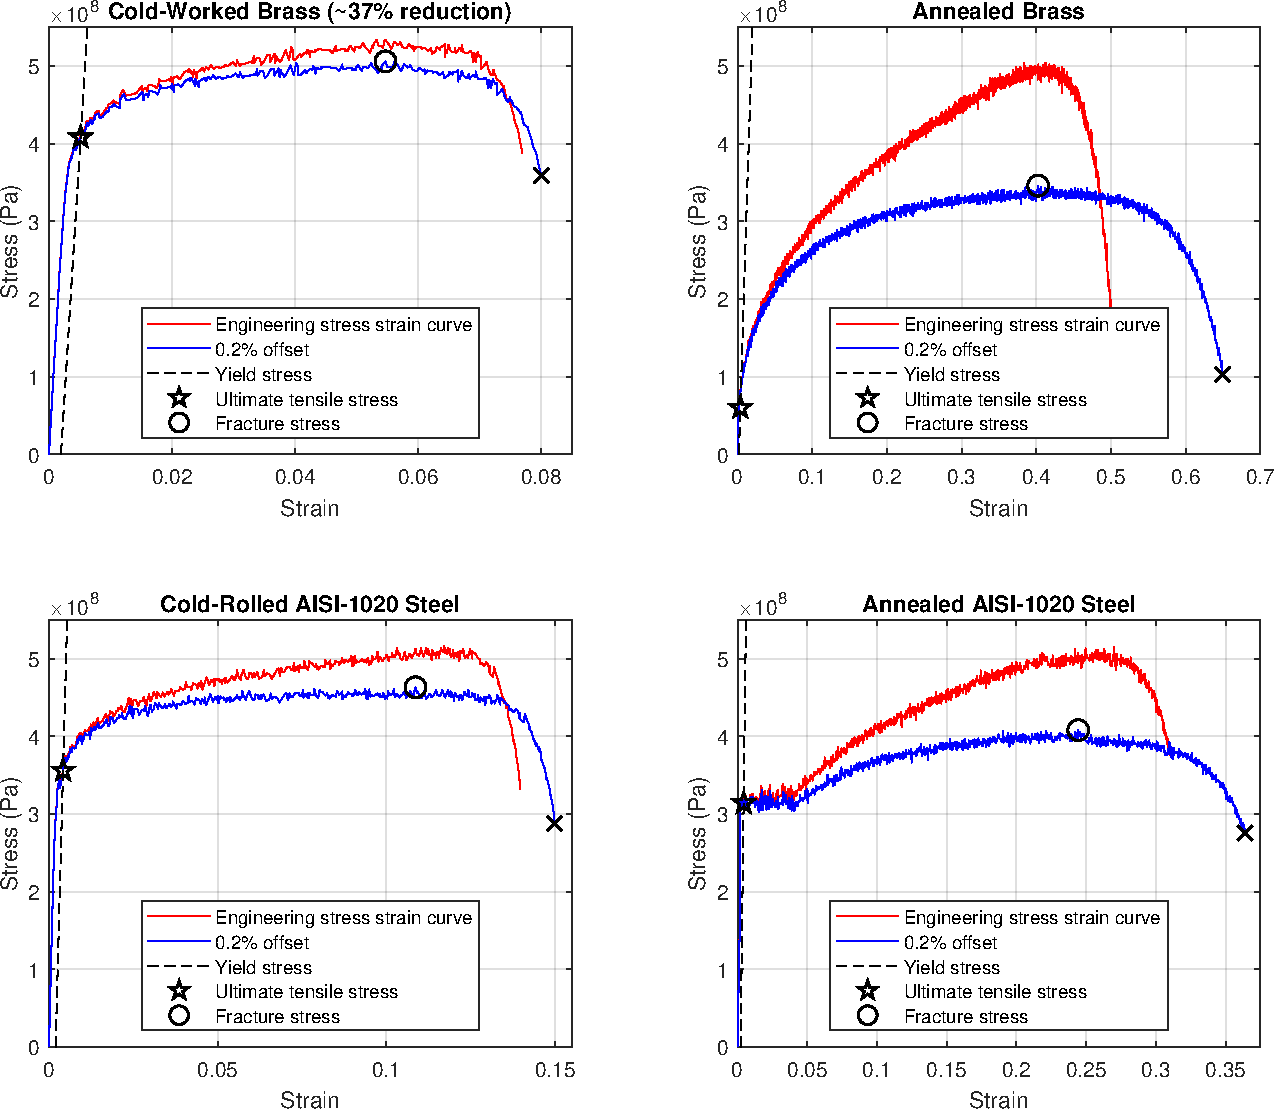
\includegraphics[width=0.9\linewidth]{metals_ss.pdf}
                \caption{Stress strain curves for all the metal specimens.}\label{fig:metals_ss}
            \end{figure}
            \begin{figure}[H]
                \centering
                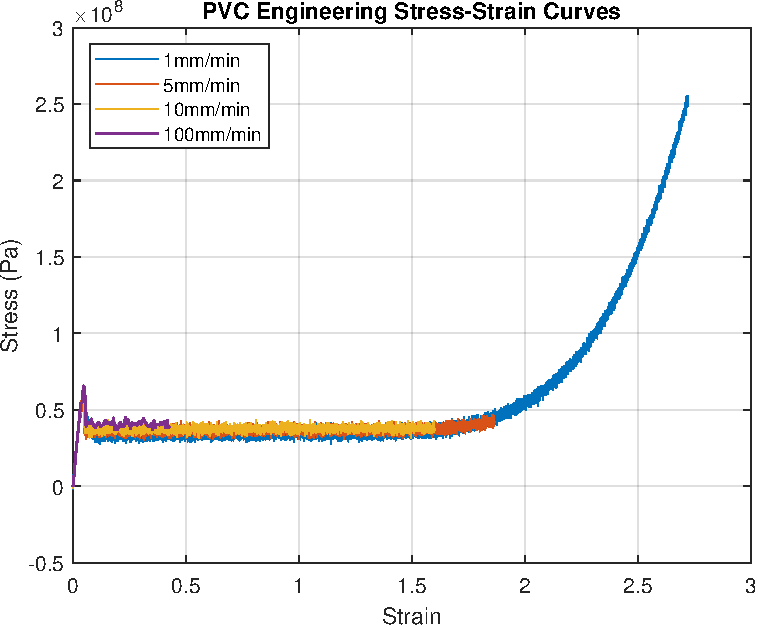
\includegraphics[width=0.5\linewidth]{pvc_ss.pdf}
                \caption{Stress strain curves for all PVS tensile testing rates.}\label{fig:pvc_ss}
            \end{figure}
        \subsection{Key mechanical properties}
            Table~\ref{tbl_brass} lists the key mechanical properties for the brass specimens. 
            Table~\ref{tbl_steel} lists the key mechanical properties for the AISI-1020 steel specimens. 
            The sample calculations and code for the key mechanical properties can be found in Appendix~\ref{code} and~\ref{sample}.
            \begin{table}[H]
                \caption{Key Mechanical Properties for Brass Specimens}
                \begin{minipage}{\linewidth}
                    \centering
                    \begin{tabular}{@{}lll@{}}
                        \toprule
                        & Cold-Worked Brass & Annealed Brass \\ 
                        \midrule
                        Young's Modulus (Experimental) & 128 GPa & 30.3 GPa \\
                        Young's Modulus (Literature)   & 117 GPa & 117 GPa \\
                        \% Difference Young's Modulus & 8.85 \% & 118 \% \\
                        Specific Stiffness & \(13.1\times10^6\ \text{m}^2\text{s}^{-2}\) & \(3.12\times10^6\ \text{m}^2\text{s}^{-2}\) \\
                        Yield Stress & 408 MPa & 59.8 MPa \\
                        Ultimate Tensile Stress & 506 MPa & 346 MPa \\
                        Failure Stress & 359 MPa & 103 MPa \\
                        \% Elongation & 8.00 \% & 64.9 \% \\ 
                        \bottomrule
                        \end{tabular}\label{tbl_brass}
                \end{minipage}
            \end{table}
            \begin{table}[H]
                \caption{Key Mechanical Properties for AISI-1020 Steel Specimens}
                \begin{minipage}{\linewidth}
                    \centering
                    \begin{tabular}{@{}lll@{}}
                        \toprule
                        & Cold-Rolled AISI-1020 Steel & Annealed AISI-1020 Steel \\ 
                        \midrule
                        Young's Modulus (Experimental) & 161 GPa & 140 GPa \\
                        Young's Modulus (Literature) & 186 GPa & 186 GPa \\
                        \% Difference Young's Modulus & 14.7 \% & 28.5 \% \\
                        Specific Stiffness & 20.4 \(10^6\text{m}^2\text{s}^{-2}\) & 17.7 \(10^6\text{m}^2\text{s}^{-2}\) \\
                        Yield Stress & 356 MPa & 314 MPa \\
                        Ultimate Tensile Stress & 463 MPa & 408 MPa \\
                        Failure Stress & 288 MPa & 276 MPa \\
                        \% Elongation & 15.0 \% & 36.4 \% \\ 
                        \bottomrule
                        \end{tabular}\label{tbl_steel}
                \end{minipage}
            \end{table}

    \section{Discussion}
    The cold-worked brass and steel are harder and more brittle compared to the annealed brass and steel. 
    Cold working involves the deformation of the materials below their recrystallization temperatures, and this deformation is known as plastic deformation. 
    It introduces defects and dislocations into the crystal lattice of the material, hindering the movement of dislocations and strengthening the material. 
    This process is also known as strain hardening. 
    While it increases the strength and hardness of the material, it also decreases ductility, causing the materials to fracture after undergoing less strain. 
    Therefore, the cold-worked versions of brass and steel could sustain a higher ultimate tensile stress without undergoing much deformation, but they could not handle as much strain as the annealed brass and steel. 
    The cold-worked materials also have a higher yield stress than the annealed materials due to strain hardening, making them less ductile. 
    Additionally, the cold-worked materials have a higher elastic modulus due to increased hardness~\cite{Lan2013}.

    The annealing process removes the dislocations and defects introduced during cold working, allowing for the rearrangement of atoms into a less strained structure. 
    This decreases the hardness of the material, making it more ductile and allowing for more plastic deformation before fracture. 
    The annealed materials also have a lower fracture stress than the cold-worked materials because they can handle more strain before fracturing. 
    Looking at the material properties of AISI-1020 steel and brass~\cite{Lin2016}\cite{Xiao2011}\cite{SAE1999}, without considering the conditions, steel is a harder and more brittle material than brass due to its higher Young's modulus. 
    This means that steel could sustain a higher stress than brass without experiencing much deformation~\cite{Douglas2014}.
    
    Annealing heats up a material, decreasing hardness and increasing ductility. 
    During annealing, a material goes through stages of recovery, recrystallization, and grain growth. 
    During recovery, a metal is heated to a temperature below the melting point, reducing the number of dislocations, increasing ductility, and reducing hardness. 
    This is shown in the results as annealed brass has a significantly lower yield stress. 
    In the recrystallization stage, the metal is further heated up, still below the melting point, forming a new grain structure, resulting in increased ductility. 
    This is reflected in the results, where annealed AISI-1020 steel has a greater \% elongation. 
    During the grain growth stage, the temperature is lowered, increasing grain size, reducing grain boundaries, resulting in more plastic deformation and increased ductility. 
    This is reflected in the results, as annealed brass has a much larger \% elongation value. 
    As strain is spread over a larger volume, it results in reduced hardness. 
    Therefore, in both brass and steel, there is a difference in mechanical properties when comparing cold-worked and annealed samples~\cite{Pan2020}.
    
    The use of materials for Kirschner wires, also known as K-wires or orthopedic pins, and artificial skin varies depending on their mechanical properties. 
    K-wires are used to stabilize and hold a fractured bone in its proper place. 
    Thus, it is important that the material has strong durability to withstand the forces and strain applied during use, meaning it would have a high yield and tensile stress. 
    It should also have a high enough stiffness to ensure a stable structure with little deformation, meaning it would have a high Young's Modulus. 
    Based on the materials tested in this lab, cold-rolled AISI-1020 steel is best suited for this application because it has high yield and ultimate tensile stress, Young's Modulus, and stiffness. 
    For artificial skin, it is important that it has high elasticity to provide flexible movement. 
    It also requires enough tensile strength to endure deformation without breaking. 
    Of the materials tested, annealed AISI-1020 steel would be best suited for artificial skin because it has a high \% elongation, a relatively low fracture stress, and high Young's Modulus~\cite{Woodroof2009}.
    
    Engineering stress is calculated by dividing the applied force by the original cross-sectional area of the material (\(\sigma = \frac{F}{A}\)), while true stress takes into account its instantaneous cross-sectional area. 
    Engineering strain is calculated by the ratio of change in length to the original length, while true strain uses the instantaneous length. 
    As force is applied to a material, the area decreases, causing true stress to continuously increase. 
    This results in a difference in the shape of the two curves: the engineering curve necks down, while the true stress-strain plot curves upwards. 
    True stress-strain curves provide a more accurate picture of the materials but have limitations as they are harder to measure, requiring knowledge of the instantaneous dimensions~\cite{Hibbeler2022}. 
    Ultimate tensile strength (UTS) is the maximum amount of stress that a material can withstand before fracture. 
    During deformation, as the instantaneous cross-sectional area can change, true stress will be larger than engineering stress, which is why UTS does not correspond to the maximum true stress.
    
    Thermoplasticity is the material property where a substance becomes plastic when heated and hardens when cooled. 
    Elastic deformation in thermoplastic materials is reversible, allowing the material to return to its original form. 
    Viscoelasticity is when a substance has both elastic and viscous properties. 
    This property is time-dependent because when temporary stress is applied, it causes temporary deformation, and when the stress is maintained, it causes permanent deformation. 
    An example of this is shown in toothpaste: when squeezed, it has higher viscosity, while it has higher elasticity when no stress is applied. 
    On a molecular level, this behavior is due to the entanglement of polymers, where high entanglement results in more elastic behavior, while disentanglement results in more viscous behavior~\cite{Kazmer2014}.
    
    In the viscoelastic region, polymers display a combination of solid and viscous behavior, which is time-dependent. 
    In this region, higher strain rates mean that the polymer has less time to undergo viscous flow, the gradual deformation of the polymer over time when there is an applied stress. 
    Within the viscoelastic region, the slope would be steeper for higher strain rates because the material would be stiffer and have less deformation. 
    In the plastic region, the stress drops while polymer chains untangle, but once they are straightened out, the tensile force is directly applied to the bonds between the polymer chains until it is strong enough to overcome the bond strength, causing fracture. 
    When the strain rate is lower, the plastic region is larger as sliding chains have more time to rearrange and reform bonds. 
    Thus, a higher strain rate will cause fracture with less strain because the faster rate of strain applies more tension quickly, not allowing the polymer chains sufficient time to recover and reform bonds, causing fracture~\cite{Poapongsakorn2011}.
    
    The main difference between metallic stress-strain curves and PVC curves is that metal curves are concave down while PVC curves are concave up. 
    There is also a flatter plastic region for PVC when compared to metals. 
    Since PVC is made of polymers that can reform links through intermolecular forces, it has a higher fracture stress, as it can withstand more stress~\cite{Douglas2014} 

    \section{Evaluation of the Lab Exercise}
        \subsection{Jamie Kang}
            Through this lab, which involved running online simulations, plotting data, and conducting data analysis, I gained a comprehensive hands-on experience that enhanced my understanding of the mechanical behavior of metals and polymers under a tensile test.
            I also gained additional insights into mechanisms such as plastic deformation, cold working, and ductility, beyond the content taught in the lectures.
            Moreover, I was able to gain new skills in data manipulation through MATLAB during the generation of results.

            \bigskip
            
\includegraphics[width=0.125\textwidth]{jamie.png}
        \subsection{Grace Hur}
            Although this lab exercise was done virtually, it effectively replicated an actual tensile testing process. 
            This allowed me to visualize the effect of stress applied to various materials and compare them.
            By answering the discussion questions and conducting additional research to explore material properties, I gained a better understanding of the mechanisms behind the results. 
            I also learned about the applications of material science on different materials and processes, such as annealing and cold working.

            \bigskip
            
\includegraphics[width=0.125\textwidth]{grace.png}
        \subsection{Myesha Zaman}
            This lab taught me how to interpret data and present it in a way that is both easy to understand and informative to the reader while being concise. 
            This skill development was particularly evident in my work on the conclusion. 
            Additionally, I learned about researching and making decisions on which background information to include, ensuring that even a person with minimal background information can understand this lab sufficiently. 
            It was also important to exclude unnecessary information that could take up precious space or confuse the reader.

            \bigskip
            
\includegraphics[width=0.25\textwidth]{myesha.png}
        \subsection{Jaime Thrower}
            Writing the discussion portion of this lab further developed my understanding of mechanical properties when looking through more of a materials science lens. 
            I initially struggled to visualize how materials worked on a molecular level and how this tied into mechanical properties. 
            However, the lab provided a more hands-on and visual learning aspect, helping me learn a lot more than I could have solely through lectures.

            \bigskip
            
\includegraphics[width=0.5\textwidth]{jaime.png}

    \addcontentsline{toc}{section}{References}
    \printbibliography{}

    \appendix

    \section{Sample MATLAB Code}\label{code}
        The following sample MATLAB code was used to generate the cold-worked brass plot of Fig.~\ref{fig:metals_ss}.
        \begin{verbatim}
% PROPTERTIES
filePath = 'cold worked brass.csv';
name = "Cold-Worked Brass (~37% reduction)";
full_range = 'A9:B252';
linear_range = 1:9;

% DIMENSIONS
d_0 = (10^-3)*12.7;
A_0 = (pi/4)*(d_0)^2;
G_0 = (10^-3)*50;

% READING DATA
data = readmatrix(filePath, 'Range', full_range);

% STROKE & LOAD
stroke = (10^-3)*data(:, 1);
load = (10^3)*data(:, 2);

% STRAIN & STRESS
eng_strain = (stroke)./(G_0);
eng_stress = (load)./(A_0);
true_strain = log(1 + eng_strain);
true_stress = (eng_stress).*(1 + eng_strain);

% LINEAR SECTION
linear_fit = polyfit(eng_strain(linear_range), eng_stress(linear_range), 1);
slope = linear_fit(1);
intercept = linear_fit(2);

% YIELD STRESS
offset = @(x) slope * (x - 0.002) + intercept;
yield_strain = fsolve(
    @(x) offset(x) - interp1(eng_strain, eng_stress, x), 
    0.004);
yield_stress = offset(yield_strain);

% MAX STRAIN & STRESS
[max_stress, max_index] = max(eng_stress);
max_strain = eng_strain(max_index);

% FRACTURE STRESS
fracture_strain = eng_strain(end);
fracture_stress = eng_stress(end);

% SS CURVE
plot(true_strain, true_stress, 'r');
hold on;
plot(eng_strain, eng_stress, 'b');
xlim([0 0.085])
ylim([0 550000000])
fplot(offset, 'k--');
plot(yield_strain, yield_stress, 'kpentagram','MarkerSize', 10, 'LineWidth', 1);
plot(max_strain, max_stress, 'ko','MarkerSize', 10, 'LineWidth', 1);
plot(fracture_strain, fracture_stress, 'kx','MarkerSize', 10, 'LineWidth', 1);
title(name);
xlabel('Strain');
ylabel('Stress (Pa)');
legend(
    'True stress strain curve', 
    'Engineering stress strain curve', 
    '0.2% offset', 
    'Yield stress', 
    'Ultimate tensile stress', 
    'Fracture stress', 
    'Location', 'south');
grid on;
hold off;
        \end{verbatim}
    \section{Sample Calculations}\label{sample}
        All sample calculations shown use values for cold-worked brass.

        \subsection{\% Difference Young's Modulus}
        \vspace*{-\baselineskip}
        \begin{align*}
            \text{\% Difference}\ E
            &= \frac{\left\vert E_{experimental} - E_{literature} \right\vert}{\frac{\left( E_{experimental} + E_{literature} \right)}{2}} \times 100 \\
            &= \frac{\left\vert(127.5098\times10^{9}\ \text{Pa}) - (116.7\times10^{9}\ \text{Pa})\right\vert }{\frac{(127.5098\times10^{9}\ \text{Pa}) - (116.7\times10^{9}\ \text{Pa})}{2}} \times 100 \\
            &= 8.8529\ \text{\%}
        \end{align*}

        \subsection{Specific Stiffness}
        \vspace*{-\baselineskip}
        \begin{align*}
            \text{Specific Stiffness}
            &= \frac{E_{experimental}}{\rho} \\
            &= \frac{(127.5098\times10^{9}\ \text{Pa})}{(9.7\ \text{g}\cdot\text{cm}^{-3})} \\
            &= 13.1453\times10^6\ \text{m}^2\text{s}^{-2}
        \end{align*}

        \subsection{\% Elongation}
        \vspace*{-\baselineskip}
        \begin{align*}
            \text{\%}\delta 
            &= \frac{(L_f - L_0)}{L_0} \\
            &= \frac{(0.0039996\ \text{m})}{(0.05\ \text{m})} \\
            & = 7.9992\ \text{\%}
        \end{align*}

\end{document}